\chapter{Literature Review}% Main chapter title
\thispagestyle{nohead}
\label{LitReview} % For referencing the chapter elsewhere, use \ref{LitReview} 

%----------------------------------------------------------------------------------------

\where incorporates ideas from at least three separate disciplines: software verification, machine learning, and software measurement and metrics. Each of these disciplines has a considerable body of research associated with it. This chapter focusses on the intersections of the three areas while addressing to relevant literature from each individual area.
A Venn diagram illustrating how the literature was classified is given in Figure \ref{fig:litreview}. It can be seen that the intersection of \textit{software verification} and \textit{measurement/metrics} itself contains two separate categories of interest: benchmarks and competitions in formal methods, and the relatively young field of \textit{proof engineering}.
The rest of this chapter will review the literature associated with each segment of Figure \ref{fig:litreview} - moving clockwise from the software verification circle.

\begin{figure}

\centering
\def\firstcircle{(3cm,0cm) circle (2.5cm)}
\def\secondcircle{(0cm,0cm) circle (2.5cm)}
\def\thirdcircle{(1.5cm,3cm) circle (2.5cm)}
% Suppose we have three circles or ellipses or whatever. Let us define
% commands for their paths since we will need them repeatedly in the
% following:
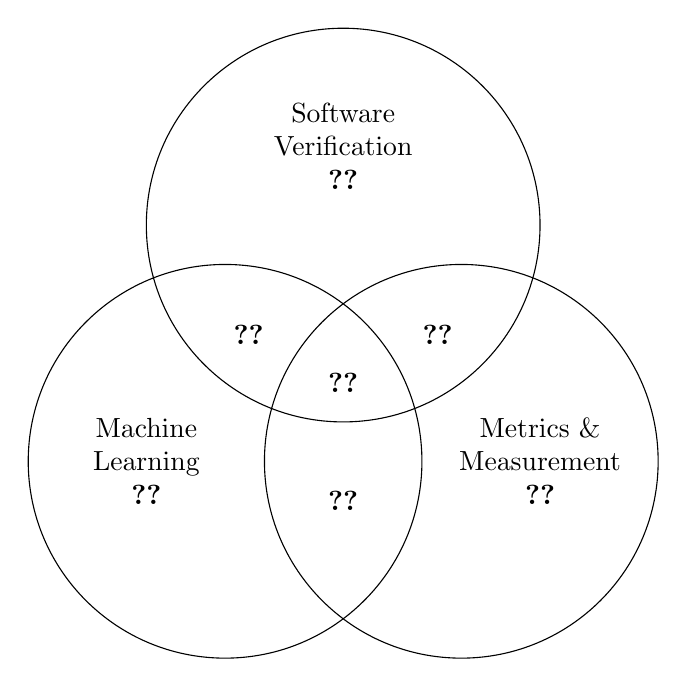
\begin{tikzpicture}
	
	\draw \firstcircle node [below] {};
	\draw \secondcircle node [above] {};
	\draw \thirdcircle node [below] {};
	\node[align=center] at (-1cm, 0cm) {Machine\\Learning\\ \ref{sec:lrml} };
	\node[align=center] at (1.5cm, 4cm) {Software\\Verification\\ \ref{sec:lrsv}};
	\node[align=center] at (4cm, 0cm) {Metrics \&\\ Measurement\\ \ref{sec:lrmm}};
	\node[align=center] at (1.5cm, 1cm) {\ref{sub:lrsvmmml}};
	\node[align=center] at (0.3cm, 1.6cm) {\ref{sub:lrsvml}};
	\node[align=center] at (2.7cm, 1.6cm) {\ref{sub:lrsvmm}};
	\node[align=center] at (1.5cm, -0.5cm) {\ref{sub:lrmmml}};
	
\end{tikzpicture}

\caption{Three disciplines identifies as being relevant to this project}
\label{fig:litreview}

\end{figure}


\section{Software Verification Systems}
\label{sec:lrsv}

To discuss the \why software verification system in relation to other comparable systems, we first look at the architecture and design of \why itself \cite{why:shephard}. The first-order logic (with polymorphic types) of the \why specification language is introduced as being flexible  


\subsection{Verification and Measurement}
\label{sub:lrsvmm}


\subsubsection{Benchmarks and Competitions}
\label{sub:lrsvmmbench}

The need for a standard set of benchmarks for the diverse range of software systems is a recurring issue in the literature \cite{Dagstuhl}. The benefits of such a benchmark suite are identified by the SMTLIB \cite{SMTLIB} project. The performance of SMT solvers has significantly improved in recent years due in part to the standardisation of an input language and the use of standard benchmark programs in  competitions \cite{SMTEVAL2013}\cite{SVCOMP}. The TPTP (Thousands of Problems for Theorem Provers) project \cite{TPTP} has similar aims but a wider scope: targeting theorem provers which specialise in numerical problems as well as general-purpose SAT and SMT solvers. The TPTP library is specifically designed for the rigorous experimental comparison of solvers \cite{Sutcliffe200139}.

\subsubsection{Proof Engineering}
\label{sub:lrsvmmpe}

\section{Software Measurement and Metrics}
\label{sec:lrmm}
%also include the experimental process

\subsection{Measurement and Machine Learning}
\label{sub:lrmmml}

\section{Machine Learning}
\label{sec:lrml}

\subsection{Verification and Machine Learning}
\label{sub:lrsvml}

\subsection{Where4 and the intersection of all three disciplines}
\label{sub:lrsvmmml}
